\documentclass[12pt]{article}
\usepackage{graphicx}
\usepackage{amsmath}
\usepackage[margin=1.0in]{geometry}
\usepackage{color, colortbl}
\usepackage{neuralnetwork}
\usepackage{hyperref}
\usepackage{float}
\usepackage[affil-it]{authblk}
\usepackage[english]{babel}
\definecolor{LightCyan}{rgb}{0.88,1,1}
\definecolor{LightRose}{rgb}{1,0.88,0.88}
\definecolor{LightGreen}{rgb}{0.88,1,0.88}

\title{Auto-encoders for Track Reconstruction in Drift Chambers for CLAS12}

\author[1]{Gagik Gavalian\thanks{Corresponding author}}
\affil[1]{Thomas Jefferson National Accelerator Facility, Newport News, VA 23606}
\date{}

\begin{document}

\begin{titlepage}
\maketitle
\begin{abstract}
In this article we describe the development of machine learning models to assist the CLAS12 tracking algorithm
by identifying tracks through inferring missing segments in the drift chambers.  Auto encoders are used to reconstruct 
missing segments from track trajectory. Implemented neural network was able to reliably reconstruct missing segment positions with accuracy of $\approx 0.35$ wires, and lead to recovery of missing tracks with accuracy of $>99.8\%$. 
\end{abstract}
\end{titlepage}

\section{Introduction}

\indent

The CLAS12\cite{Burkert:2020akg} detector is built around a six-coil toroidal magnet which divides the active detection into six azimuthal regions, called "sectors". The torus coils are approximately planar. Each sector subtends an azimuthal range of 60$^\circ$ from the mid-plane of one coil to the mid-plane of the adjacent coil. The “sector mid-plane” is an imaginary plane which bisects the sector’s azimuth. 
Charged particles in the CLAS12 detector are tracked using drift chambers\cite{Mestayer:2020saf} inside the toroidal magnetic field. There are six identical independent drift chamber systems in CLAS12 (one for each azimuthal sector). Each sector of drift chambers consists of three chamber sets (called "regions"), and each region consists of two chambers called super-layers each of them containing 6 layers of wires perpendicular to particle trajectories in CLAS12. The tracks passing through drift chambers leave signal in each of the layers (36 in total), which are broken down into 6 segments (one segment per super-layer). The tracking algorithm relies on forming track candidates on all combinations of segments (one from each super-layer).
With time some inefficiencies in detector develop leading to missing segments in one (or more) of the super-layers, and this results in efficiency drop in track identification. In this work we investigate neural networks that can help as improve the track finding efficiency when there are missing segments in some parts of the drift chambers.

\section{Reconstruction Procedure}

\indent

Particle traveling through drift chambers leaves signal in each of the 36 planes in the path of particle. The signals in each super-layer are combined into segments. On Figure~\ref{dc:display} examples event are shown, where the horizontal lines on the plot correspond to boundaries of each super-layer. The tracking algorithm constructs track candidates from composed segments by requiring one segment per super-layer for each track candidates. Each track candidate is fitted using Kalman-Filter to reconstruct a track, and depending on convergence it's either disregarded or marked as good track for further considerations. This process of track candidate fitting is computationally intensive, and we already developed a neural network for CLAS12~\cite{Gavalian:2020oxg} detector which identifies correct combinations of segments to be considered by tracking algorithm. The developed network provided accuary of $>99.7\%$ and accelerated tracking code by factor of 6, by composing possible track candidate list using neural network.

\begin{figure}[!ht]
\begin{center}
 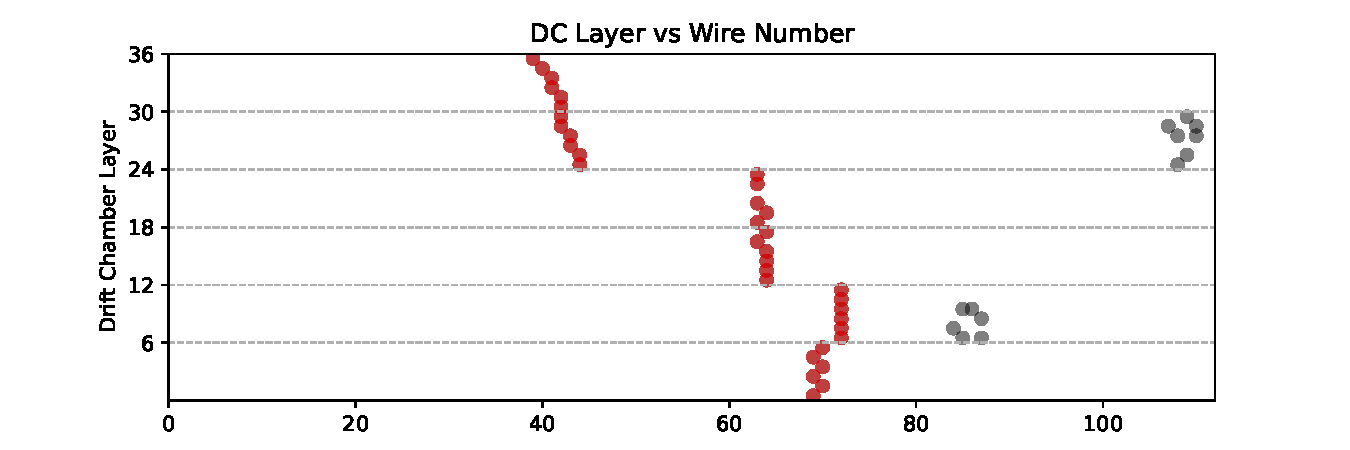
\includegraphics[width=3.2in]{images/figure_raw_20.pdf}
 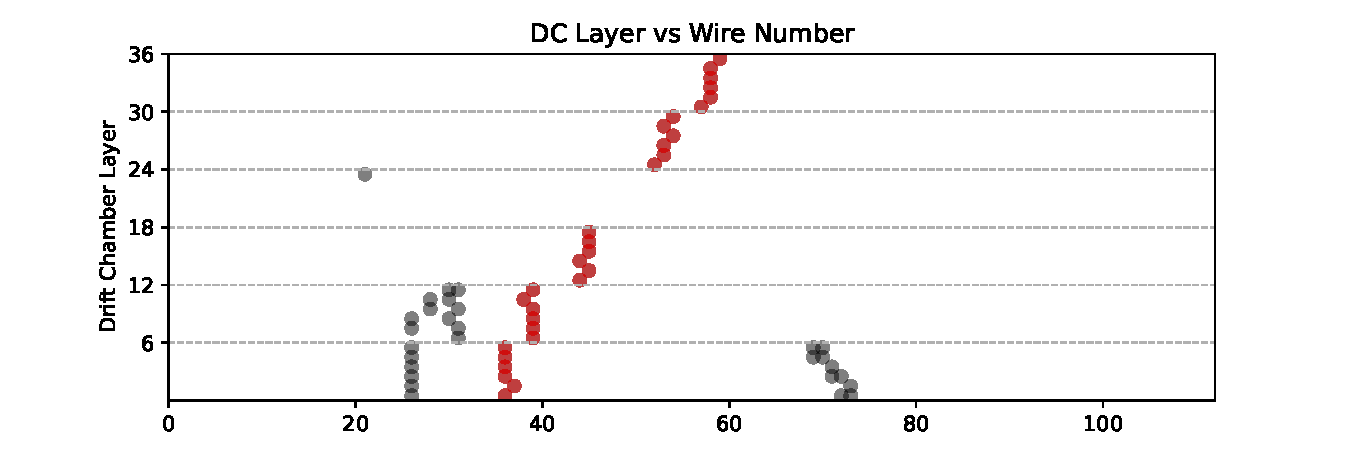
\includegraphics[width=3.2in]{images/figure_raw_22.pdf}
  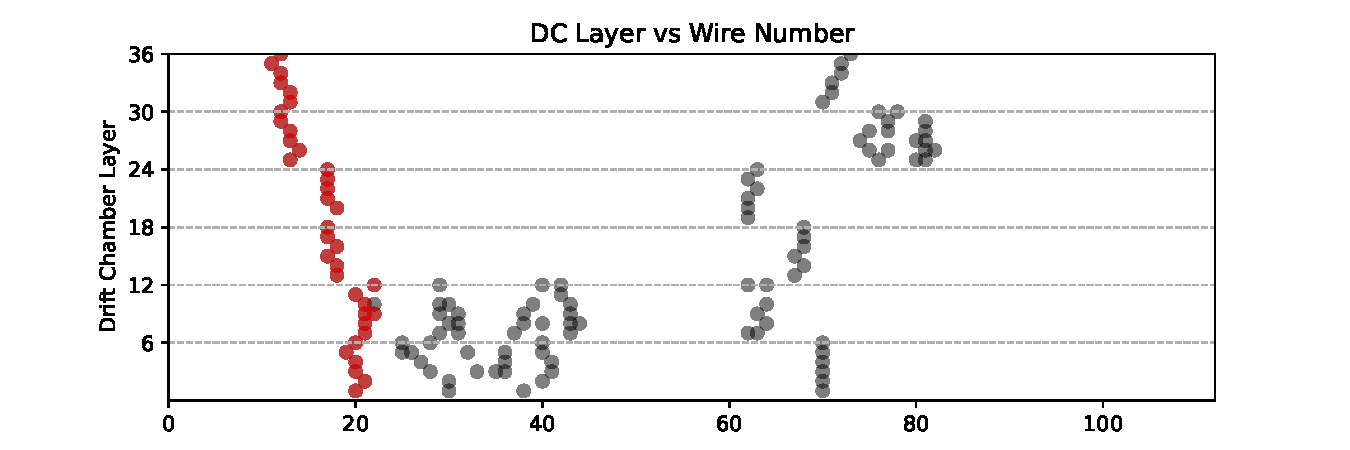
\includegraphics[width=3.2in]{images/figure_raw_21.pdf}
   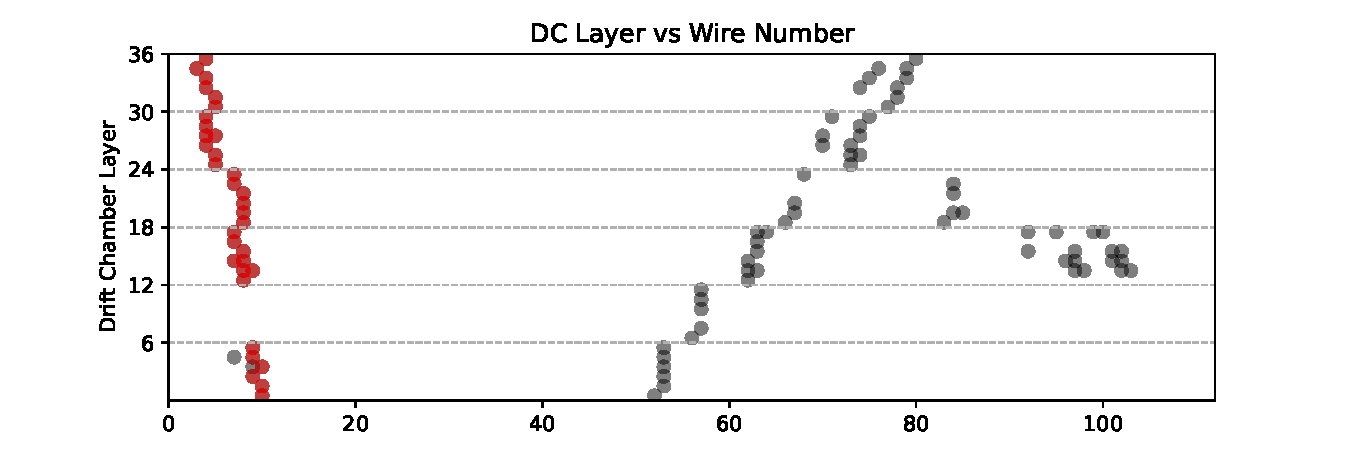
\includegraphics[width=3.2in]{images/figure_raw_23.pdf}
\caption {Events from one of the sectors of drift chambers, where background hits (in gray) are plotted along with 
reconstructed track segments (red points). Events in the left column have all six segments present in the track, events
in the right column have one of the segments missing. The dashed lines on the plot show super-layer boundaries.}
 \label{dc:display}
 \end{center}
\end{figure}

This procedure works well when all 6 super-layers have segment on the particle path. But with time drift chambers develop regions where efficiency of producing signal in the wire drops, and it is possible to end up with only 5 segments on the particle path, example of these events can be seen on Figure~\ref{dc:display} (right column). The current algorithm for track candidate identification classifier relies on 6 segment combinations to correctly identify tracks.

When missing segments are in the first or last super-layer series prediction can be successfully used to predict last missing segment given 5 consecutive segments. We have already developed a series prediction neural network (using LSTMs)~\cite{Angelopoulos20P} capable of predicting last missing segment. 

However, the missing segment can appear in any of the super-layers, and we need a reliable way of predicting missing segment location, in order to pass complete track candidate information to our classifier network, which in turn can decide if the track is a valid track. To solve this problem we decided to use auto-encoder type network.

\section{Network Architecture}

\indent

An auto-encoder is an unsupervised learning technique for neural networks that learns efficient data representations (encoding) by training the network to ignore signal “noise.” 
The auto-encoder network has three layers: the input, a hidden layer for encoding, and the output decoding layer. Using back-propagation, the unsupervised algorithm continuously trains itself by setting the target output values to equal the inputs. This forces the smaller hidden encoding layer to use dimensional reduction to eliminate noise and reconstruct the inputs.
Auto-encoder networks teach themselves how to compress data from the input layer into a shorter code, and then uncompress that code into whatever format best matches the original input. This process sometimes involves multiple autoencoders, such as stacked sparse auto-encoder layers used in image processing.

There are several types of auto-encoders:

{\bf De-noising auto-encoders:}  Using a partially corrupted input to learn how to recover the original undistorted input.
 More hidden encoding layers than inputs, and some use the outputs of the last auto-encoder as their input.

{\bf Contractive auto-encoder} : This uses an explicit “regularizer” that forces the model to learn a function that is robust against different variations of the input values.

\begin{figure}[!ht]
\begin{center}
 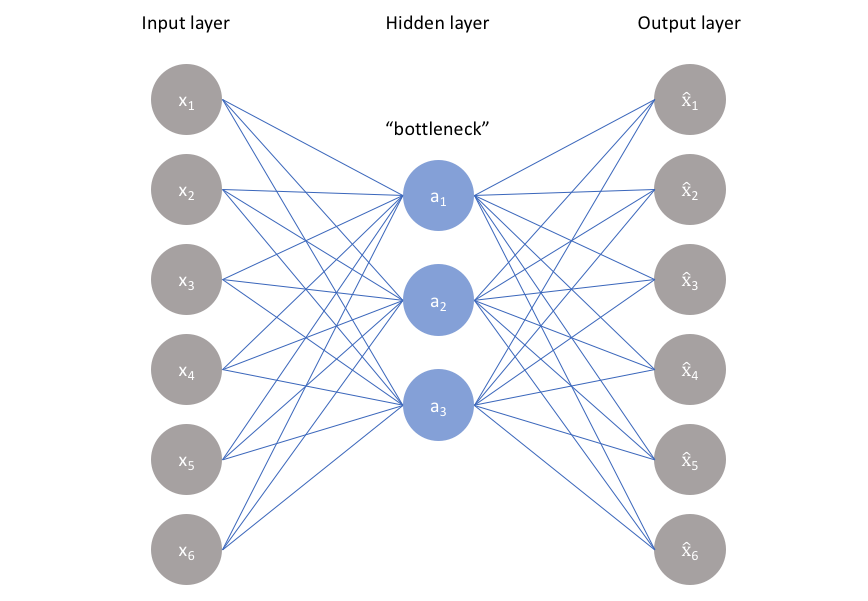
\includegraphics[width=3.0in]{images/ae_nb.png}
 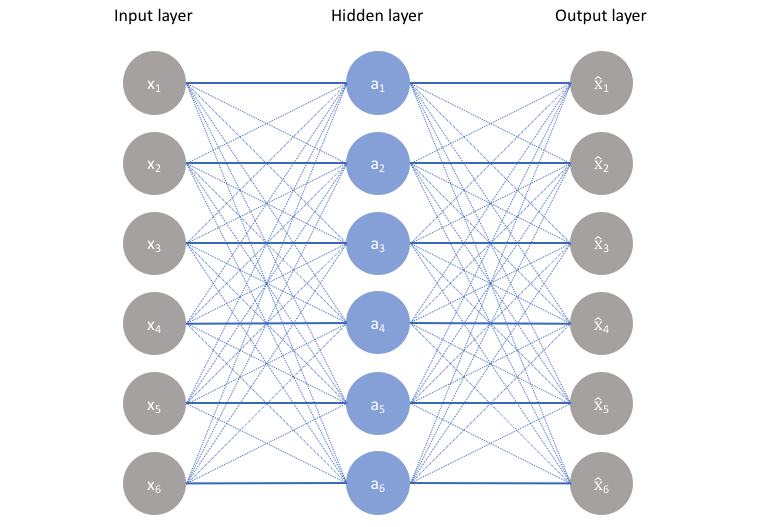
\includegraphics[width=3.0in]{images/ae_b.png}
\caption {Auto-encoder neural network architecture types.}
 \label{pic:autoencoders}
 \end{center}
\end{figure}

On Figure~\ref{pic:autoencoders}) different architectures of auto-encoder can be seen. For this study we used 
an auto-encoder with structure show in Table~\ref{table:network}. Several different configurations were tried, and
we discovered this one to provide the best accuracy.
The network was implemented in Java using machine learning library Neuroph~\cite{neuroph-2.98}. 

\begin{table}[!h]
\begin{center}
\begin{tabular}{|l|c|c|c|c|c|}
\hline
 & Input Layer & Hidden Layer 1 & Hidden Layer 2 & Hidden Layer 3 & Output Layer \\
\hline
\hline
Type & Dense Layer & Dense Layer &Dense Layer &Dense Layer &Dense Layer \\
\hline
Nodes & 6 & 12 & 6 & 12 & 6 \\
\hline
\end{tabular}
\end{center}
\caption{Neural Network architecture for resolving missing segments from track data.}
\label{table:network}
\end{table}

With this network we plan to recover missing segment information. The input to the network is
the average wire position of each segment in for of a vector:

\begin{equation}
X = {x_1,x_2,x_3,x_4,x_5,x_6}
\end{equation}

There the index is the super-layer number for each segment, and the value is:

\begin{equation}
x_k = \sum_{i=1..N} \frac{w^k_i}{N}
\end{equation}

where N is number of hits in the segment, and $w^k_i$ is the wire position of the hit $i$
in super-layer $k$. And the output provided to the network is:

\begin{equation}
Y = (x_1,x_2,x_3,x_4,x_5,x_6)
\end{equation}

The corruption was introduced in the input set of training data by setting one of the values of the vector to "0",
and neural network was trained to reconstruct the input data in the output without corruption. The procedure
of data corruption is discussed in the next section.


\section{Data Selection}
\label{section:data}

\indent

For this study we selected events from processed data where a track was reconstructed in a given
sector and contained segments from all 6 super-layers. The input data set is a vector of 6 values,
representing the mean wire positions for each segment in given super-layer:

\begin{equation}
 X = (x_1,x_2,x_3,x_4,x_5,x_6)
\end{equation}

and the output vector is contains the same values as input:

\begin{equation}
Y ={x_1,x_2,x_3,x_4,x_5,x_6}
\end{equation}

Two data sets were composed from this initial sample. One with one of the values of input vector set to "0.0"
(chosen randomly):

\begin{equation}
  (x_1,x_2,x_3,x_4,x_5,x_6) \begin{cases}
    i = rndm(1..6)  & x_i = 0.0  \\
    X (x_1,0.0,x_3,x_4,x_5,x_6)   \text{$\rightarrow$}  & Y (x_1,x_2,x_3,x_4,x_5,x_6) \\
     \end{cases}
\end{equation}

In this given case i=2. For the second training set, each sample of X,Y vectors
was extended to 6 samples where in each sample one of the input vector values 
was set to "0.0":

\begin{equation}
  (x_1,x_2,x_3,x_4,x_5,x_6) \begin{cases}
   X (0.0,x_2,x_3,x_4,x_5,x_6)  \text{$\rightarrow$}  & Y (x_1,x_2,x_3,x_4,x_5,x_6)  \\
   X (x_1,0.0,x_3,x_4,x_5,x_6)   \text{$\rightarrow$}  & Y (x_1,x_2,x_3,x_4,x_5,x_6) \\
   X (x_1,x_2,0.0,x_4,x_5,x_6)  \text{$\rightarrow$}  &  Y (x_1,x_2,x_3,x_4,x_5,x_6) \\
   X (x_1,x_2,x_3,0.0,x_5,x_6)  \text{$\rightarrow$}  & Y (x_1,x_2,x_3,x_4,x_5,x_6) \\
   X (x_1,x_2,x_3,x_4,0.0,x_6)  \text{$\rightarrow$}  & Y (x_1,x_2,x_3,x_4,x_5,x_6) \\
   X (x_1,x_2,x_3,x_4,x_5,0.0)  \text{$\rightarrow$}  & Y (x_1,x_2,x_3,x_4,x_5,x_6)
  \end{cases}
\end{equation}

The second training sample is just ensuring that all combinations of missing segment information
is represented in the training sample. If very large data set is used for training the first method of data
construction should be sufficient since many combinations of similar tracks with random number of missing
segments randomly removed will be represented in training set in abundance.


\section{Results}

\indent

For this study we used tracks reconstructed with conventional algorithm and trained network using two data sets
(described in section \ref{section:data}). Training sample consisted of 5,000 samples, and testing sample was 3,500 samples
(testing sample was different from training sample). Two networks were trained and evaluated for this study. One with using random substitution in input training set and one with creating 6 individual input and output pair for each input data sample.
Then trained network was used to evaluate the testing data set. From testing data set one of the nodes was set to "0.0", choosing node randomly then the vector was provided as an input for trained network and in from the output the value for that particular element of the vector was compared to the value of same element in the input vector.

\begin{figure}[!ht]
\begin{center}
 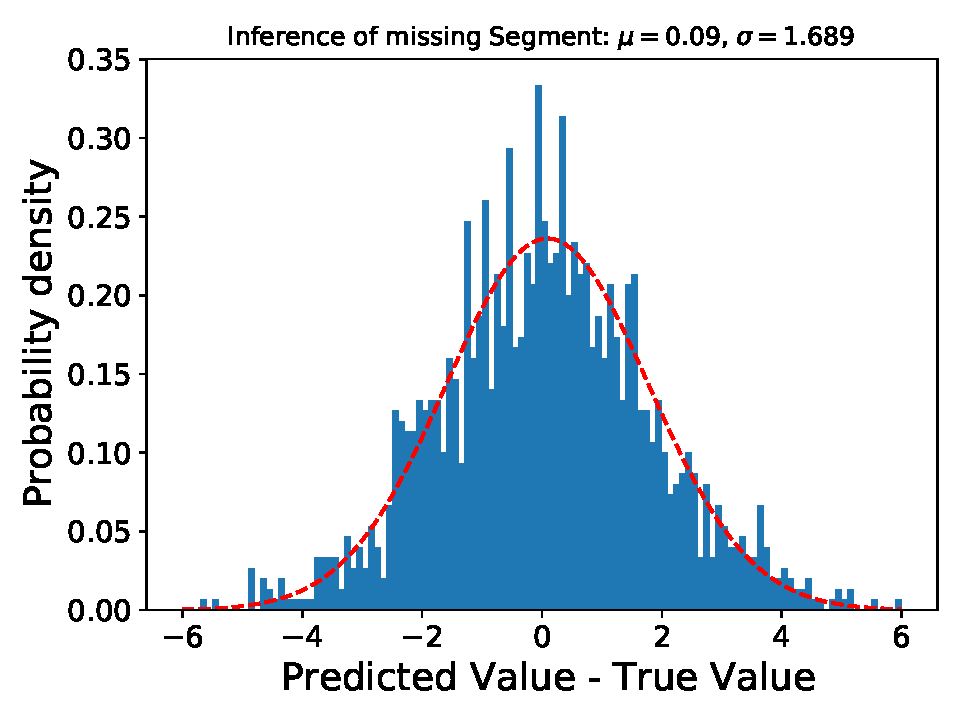
\includegraphics[width=3.0in]{images/figure_r.pdf}
 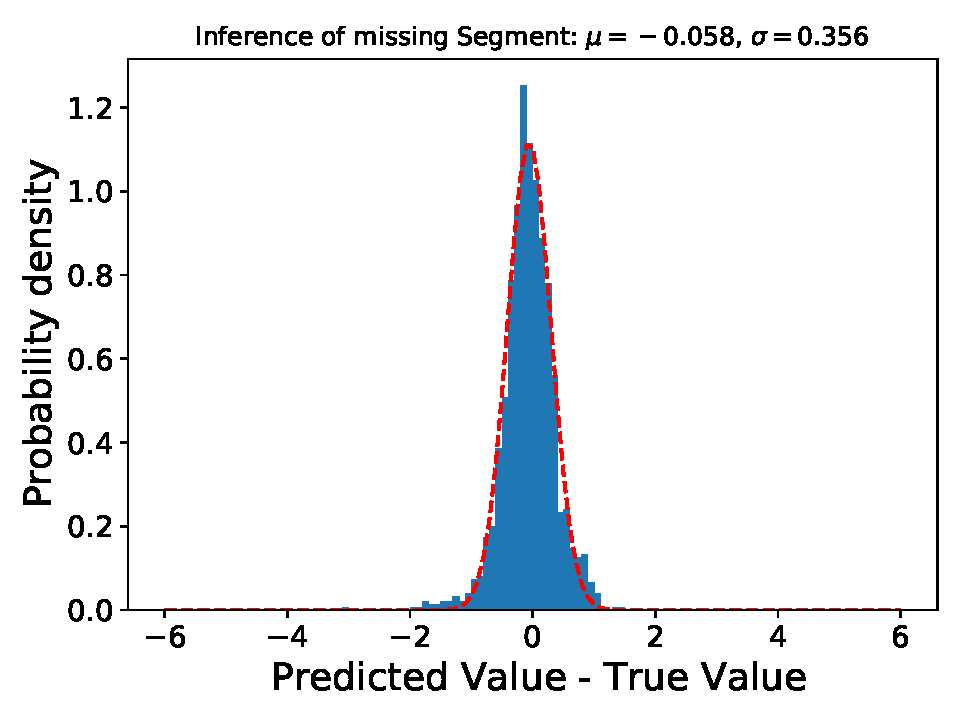
\includegraphics[width=3.0in]{images/figure_n.pdf}
\caption {Results of Neural Network Performance. The missing segment average wire numbers were inferred using trained network and the difference with plotted for regular data set (on the left) and extended data set (on the right). }
 \label{ml:results}
 \end{center}
\end{figure}

The results of network evaluation is shown on Figure~\ref{ml:results}, where performance of both networks is presented with the corresponding fit. On Figure~\ref{ml:results} (left) the performance of network trained with random "0.0" substitutions is presented, the difference between "True" segment value vs inferred segment mean value is plotted. The average uncertainty of inference is $1.7$ wires. On Figure~\ref{ml:results} (right) the performance of second network is shown with much better performance with uncertainty of $0.36$ wires. On Figure~\ref{ml:results2d}  the performance of two networks are shown as a function of which corrupt node that was reconstructed by network. There are some systematic shifts depending on the knocked out node, but they are well within the average error.

\begin{figure}[!ht]
\begin{center}
 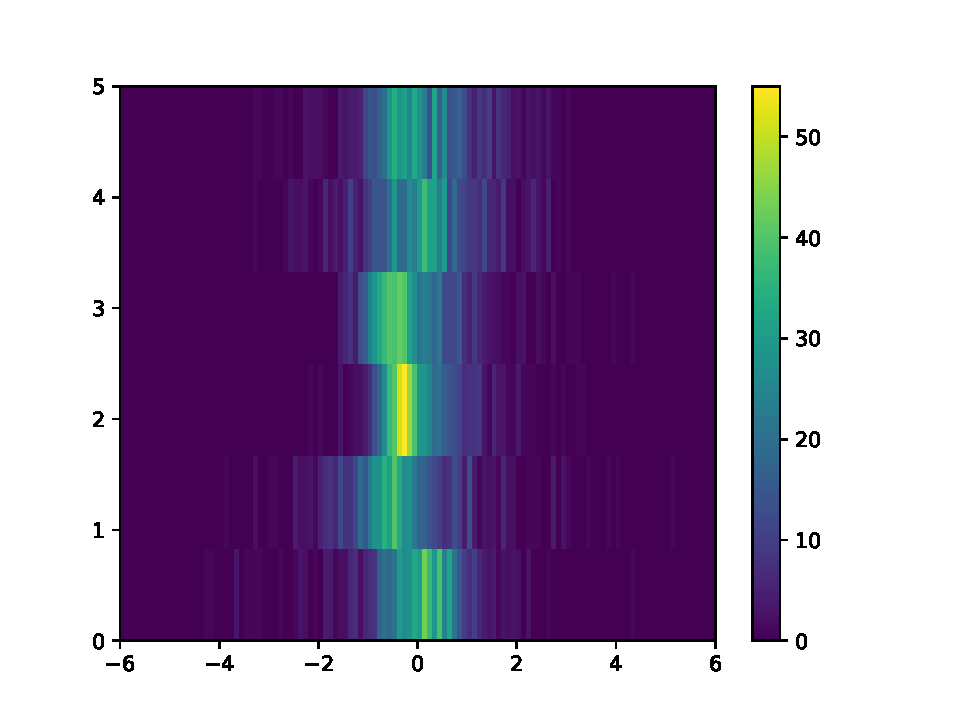
\includegraphics[width=3.0in]{images/figure_2d_r.pdf}
 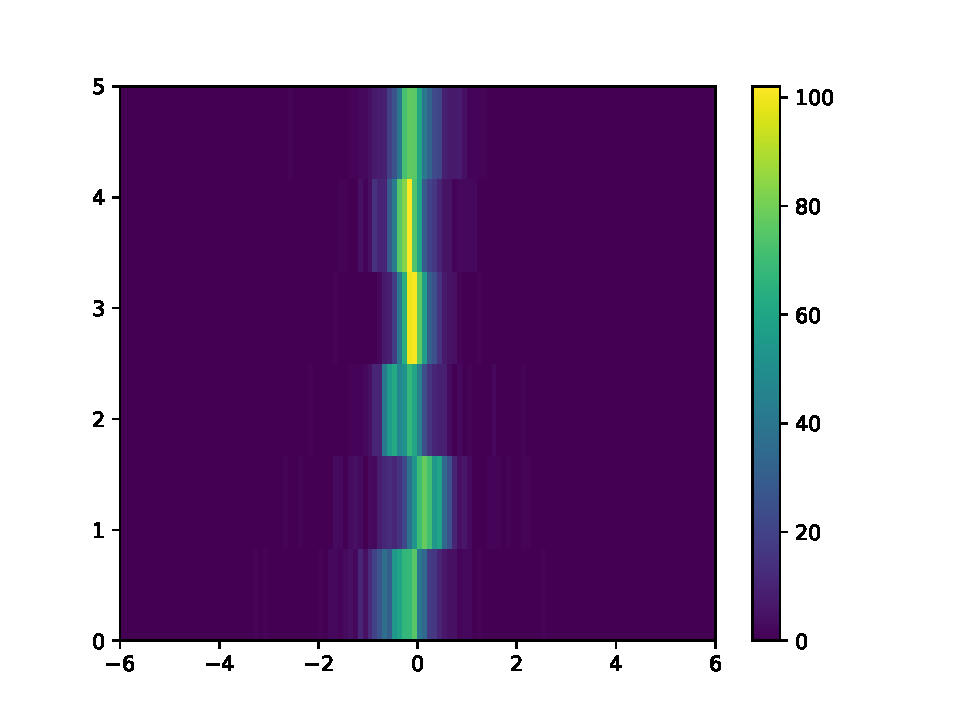
\includegraphics[width=3.0in]{images/figure_2d_n.pdf}
\caption {Performance of neural network missing segment inference as a function of missing segment trained with regular data  set (on the left) and with extended data set (on the right).}
 \label{ml:results2d}
 \end{center}
\end{figure}

In theory with increasing training sample the performance of first network should asymptotically reach performance of second network which has more complete training sample, and the procedure of extending training sample will not be necessary. We extended the training sample by duplication to overcome sparsity of data sameple, and to illustrate that this technique works
with smaller training sample.

\newpage
\bibliography{references}
\bibliographystyle{ieeetr}

\end{document}
